\chapter{Fragen zur Vorbereitung}
\section{Wichtige Daten und Gegenkopplung eines Operationsverstärkers}
\textbf{Welche wichtigsten Daten hat ein idealer und welche ein realer Operationsverstärker?\\
Wie verändert die Gegenkopplung den Frequenzgang des Operationsverstärkers und
was bedeutet in diesem Zusammenhang das \textit{Verstärkung–Bandbreite–Produkt}?}

Wichtige Daten für den Operationsverstärker sind die Verstärkung ($\nu$), der Ein-\- und Ausgangswiderstand (\(R_\text{e}$, $R_\text{a}\)) und die Einstellzeit ($\tau$) des Ausgangssignals.\\
Bei einem idealen Operationsverstärker sollte die Verstärkung (Verhältnis von Ausgangsspannung zu Eingangsspannung) ziemlich groß sein.
Der Eingangswiderstand sollte so hochohmig wie möglich sein, um die Signalquelle nicht zu belasten.
Der Ausgangswiderstand sollte dagegen so niedrig wie möglich sein, damit die Ausgangsspannung unabhängig vom angeschlossenen Verbraucher ist.
Die Einstellzeit sollte so klein wie möglich sein, damit das Ausgangssignals dem Eingangssignal nahe zu verzögerungsfrei folgt und hohe Frequenzen können problemlos verstärkt werden.
Außerem soll der Operationsverstärker ein Ausgangssignal von $0\,\text{V}$ ausgeben, wenn kein Eingangssignal anliegt.\\
Somit ergibt sich folgende Gegenüberstellung eines idealen Operationsverstärker und eines realen Operationsverstärker des Typs \textbf{CA 3140} \citep[vgl.][S.259]{EKS}:
\begin{table}[h]
    \centering\begin{tabular}{c|c|c}
        &idealer Operationsverstärker & Operationsverstärker Typ CA 3140\\
        \hline
        Verstärkung ($\nu$)&$\to \infty$&$10^5$\\
        Eingangswiderstand ($R_\text{e}$)&$\to \infty$&$1,5\cdot10^{12}\,\Omega$\\
        Ausgabgswiderstand ($R_\text{a}$)&$\to 0$&$60\,\Omega$\\
        Einstellzeit ($\tau$)&$\to 0$&$0,22\,\mu\text{s}$
    \end{tabular}
    \caption{Wichtige Daten eines idealen und realen Operationsverstärker.}
\end{table}\\
Ein Operationsverstärker kann einen ungegrenzten Frequenzbereich (Bandbreite) gleichmäßig verstärken.
Durch eine Gegenkopplung, wird die Spannungsverstärkung vermindert und kann auf eine höhere Bandbreite ausgedehnt werden, damit der Eingangswiderstand der gegengekoppelten Schaltung abnimmt \citep[vgl.][S.206]{HBG}.
Ab einer Grenzfrequenz, nimmt die Verstärkung mit steigender Eingangsfrequenz ab.
Das Produkt aus der Verstärkung und der Bandbreite nennt man das Verstärkung–\-Bandbreite–Produkt (\(b\cdot\nu\)).
Dieses ist bei der Abnahme der Verstärkung konstant und eine Kenngröße des Operationsverstärkers, welche man in Schaltungen ausnutzen, aber nicht überschreiten kann \citep[vgl.][S.206]{HBG}.\newpage
\section{Begriffserklärungen}
\textbf{Erklären Sie kurz die Bedeutung der folgenden Begriffe: Eingangs–Offsetstrom,
Eingangs–Offsetspannung, Gleichtakt–Eingangswiderstand, Differenz–Eingangswiderstand, Gleichtakt–Eingangsbereich, Differenz–Eingangsbereich, Slewrate.\\
Was ist mit \textit{Impedanzwandlung} gemeint und wofür ist das wichtig?}
\begin{description}
    \item[Eingangs–Offsetstrom:] Bezeichnet die Differenz der beiden Eingangsströme bei der die Ausgangsspannung $0\,\text{V}$ wird \citep[vgl.][S.408]{HBG}.
    \item[Eingangs–Offsetspannung:] Bezeichnet die angelegte Eingangsspannung des Operationsverstärkers bei der die Ausgangsspannung $0\,\text{V}$ ist \citep[vgl.][S.408]{HBG}.
    \item[Gleichtakt–Eingangswiderstand:] Diese Widerstände liegen zwischen den jeweiligen Eingang und der Masse an. Diese sind parallel zu den Eingängen geschalten und werden durch die Gegenkopplung nicht beeinflusst. Der Widerstand am nichtinvertierenden Eingang sorgt für eine Abschwächung und der am invertierten Eingang für eine Verstärkung des Signals. Diese Effekte lassen sich kompensieren, wenn beide Signale im Operationsverstärker abgeglichen sind \citep[vgl.][]{wiki-op}.
    \item[Differenz–Eingangswiderstand:] Dieser Widerstand liegt zwischen dem invertierden und nichtinvertierden Eingang an und wird durch die Gegenkopplung stark erhöht. Somit wird die Spannung zwischen den beiden Eingängen bei $0\,\text{V}$ gehalten \citep[vgl.][]{wiki-op}.
    \item[Gleichtakt–Eingangsbereich:] Bezeichnet den Bereich der maximalen Eingangsspannungen, in der der Operationsverstärker ordnungsgemäß arbeitet \citep[vgl.][]{ees}.
    \item[Differenz–Eingangsbereich:] Bezeichnet die Differenz der zulässigen Eingangsspannungen, indem der Operationsverstärker normal arbeitet \citep[vgl.][]{ees}.
    \item[Slewrate:] bezeichnet die durch bauartbedingte schnellste Änderung der Ausgangsspannung \citep[vgl.][S. 409]{HBG}.
\end{description}
Der Impedanzwandler transformiert den hohen Eingangswiderstand auf niedrigen Ausgangswiderstand.
Da mit dem Operationsverstärker meist Wechselströme verstärkt werden, sind diese Widerstände, Schein-Widerstände oder Impedanzen \citep[vgl.][S. 260]{EKS}.\newpage
\section{Nichtinvertierender Verstärker}
\textbf{Zeigen Sie, dass für den nichtinvertierenden Verstärker Gl. (4) gilt!}\\
Der nichtinvertierende Verstärker ist wie folgt aufgebaut:
\begin{figure}[h]
    \centering\begin{circuitikz}[european resistors]
        \draw(0,0) node[op amp, yscale=-1] (opamp){};
        \draw (opamp.+) to [short,-o,i_<=$I_4$] ++(-3,0) to [open,v>=$U_\text{e}$] ++(0,-4) to [short,o-] ++(2,0) to node[ground](gnd){} ++(0,0);
        \draw (opamp.-) to [short,i<=$I_3$] ++(-1,0) to [short] ++(0,-1) to node[short,*-*](r2){} ++(0,0) to [R=$R_1$,*-*,i>=$I_1$] (gnd);
        \draw (gnd) to [short,-o]++(5.35,0) to node[short,-o](end){}++(0,0);
        \draw (opamp.out) to node[short,*-*](r1){} ++(1,0) to [short,-o] ++(1,0) to [open,v>=$U_\text{a}$] (end);
        \draw (r1) to [short,*-,i>^=$I_2$]++(0,-1.5) to [R=$R_2$,v>=$U_2$] (r2);
        \draw (r2)++(0,1) to [open] ++(-1,0) to node[short](o1){} ++(0,0)to[open,v>=$U_1$]++(0,-3);
        \draw (o1) to [open,v^<=$U_3$]++(0,1);
    \end{circuitikz}
    \caption{Schaltplan des nichtinvertierenden Verstärkers.}
\end{figure}\\
Im Folgenden wird gezeigt, dass sich die Verstärkung wie folgt berechnen lässt:
\begin{equation}
    \nu=1+\frac{R_2}{R_1}
\end{equation}
Im Skript (S. 2) werden folgende Annahmen gemacht:
\begin{align}
    U_\text{e}&=U_1\\
    I_3&=I_4=0\,\text{A}
\end{align}
Mit den Kirchhoffschen Gesetze folgt:
\begin{align}
    U_1&=0\,\text{V}\\
    U_\text{a}&=U_1+U_2\\
    I_2&=I_1+I_3\\
    I_1&=I_2=I
\end{align}
Mit dem Ohm'schen Gesetzt folgt für die Verstärkung $\nu$:
\begin{align}
    \nu&=\frac{U_\text{a}}{U_\text{e}}\\
    \nu&=\frac{\left(U_1+U_2\right)}{U_1}\\
    \nu&=\frac{\left(R_1\cdot I\right)+\left(R_2\cdot I\right)}{R_1\cdot I}\\
    \nu&=\frac{R_1\cdot I}{R_1\cdot I}+\frac{R_2\cdot I}{R_1\cdot I}\\
    \nu&=1+\frac{R_2}{R_1}
\end{align}\newpage
\section{Integrationsschaltung}
\textbf{Durch die Integrationsschaltung in Abb. El2.4(a) werden Funktionsverläufe elektrischer Größen über die Zeit integriert.\\
Zeigen Sie, dass
\(U_a(T)=-\frac{1}{R_1C_2}\int_0^TU_e(t)dt+U_0\)
gilt. Wodurch wird $U_0$ festgelegt?\\
Berechnen Sie die Frequenzabhängigkeit der Verstärkung und stellen Sie diese doppeltlogarithmisch dar. Wie ändert sich der Frequenzgang, wenn Sie R2 aus Abb.
El2.5(a) berücksichtigen?\\
Skizzieren Sie dies ins gleiche Diagramm. Was muss also für die Frequenz der zu integrierenden Eingangsspannung gelten?}\\
Die Integrationsschaltung ist wie folgt aufgebaut:
\begin{figure}[h]
    \centering\begin{circuitikz}[european resistors]
        \draw(0,0) node[op amp, yscale=-1] (opamp){};
        \draw (opamp.+) to [R=$R_1$,-o,i_<=$I_1$] ++(-3,0) to [open,v>=$U_\text{e}$] ++(0,-3) to [short,o-] ++(2,0) to node[ground](gnd){} ++(0,0);
        \draw (opamp.-) to [short] ++(-1,0) to [short] ++(0,-1) to node[short](r2){} ++(0,0) to [short,-*] (gnd);
        \draw (gnd) to [short,-o]++(5.35,0) to node[short,-o](end){}++(0,0);
        \draw (opamp.out) to node[short,*-*](r1){} ++(1,0) to [short,-o] ++(1,0) to [open,v>=$U_\text{a}$] (end);
        %\draw (r1) to [short,*-,i>^=$I_2$]++(0,-1.5) to [R=$R_2$,v>=$U_2$] (r2);
        %\draw (r2)++(0,1) to [open] ++(-1,0) to node[short](o1){} ++(0,0)to[open,v>=$U_1$]++(0,-3);
        %\draw (o1) to [open,v^<=$U_3$]++(0,1);
        \draw (opamp.out) to [short,*-]++(0,2) to [C=$C_2$,i>=$I_2$]++(-2.35,0) to [short,-*] (opamp.+);
    \end{circuitikz}
    \caption{Schaltplan der Integrationsschaltung.}
\end{figure}\\
Aus den Annahmen der vorherigen Aufgabe geht hervor:
\begin{align}
    I_1+I_2&=0\,\text{A}
\end{align}
Da der Stromfluss durch den Kondensator eine zeitliche Änderung seiner Ladung beschreibt folgt:
\begin{align}
    I_2&=\frac{d}{dt}Q_{\text{C}_2}\\
    I_2&=\frac{d}{dt}\left(C_2\cdot U_\text{a}\right)\\
    I_2&=C_2\cdot\frac{d}{dt}U_\text{a}\\
    I_2&=C_2\cdot\dot{U}_\text{a}
\end{align}
Somit folgt mit dem Ohm'schen Gesetzt:
\begin{align}
    I_1&=-I_2\\
    \frac{U_\text{e}}{R_1}&=-C_2\cdot\dot{U}_\text{a}\\
    \dot{U}_\text{a}&=-\frac{1}{C_2\cdot R_1}\cdot U_\text{e}\\
    U_\text{a}(T)-\underbrace{U_{\text{a}}(0)}_{=U_0}&=-\frac{1}{R_1\cdot C_2}\cdot\int_0^T U_\text{e}(t)dt\\
    U_\text{a}(T)&=-\frac{1}{R_1\cdot C_2}\cdot\int_0^T U_\text{e}(t)dt+U_0
\end{align}
$U_0$ ist die Spannung, welche beim Zeitpunkt $t=0$ an der Ausgangsseite der Integrationsschaltung anliegt.\\

Nun soll die Frequenzabhängigkeit der Verstärkung berechnet werden. Dazu wird für die weiteren Rechnungen \(U_\text{e}(t)=U_\text{e,0}\cdot e^{i\omega t}\), mit der Anfangsbedingung $U_e(0)=0\,\text{V}$ verwendet.\\
Somit folgt für die Ausgangsspannung:
\begin{equation}
    U_\text{a}=-\frac{1}{R_1\cdot C_2}\frac{1}{i\omega}\cdot U_\text{e,0}\cdot e^{i\omega t}+\underbrace{U_0}_{=0\,\text{V}}
\end{equation}
Somit folgt für die Verstärkung:
\begin{align}
    \nu(\omega)&=\left|\frac{U_\text{a}}{U_\text{e}}\right|\\
    \nu(\omega)&=\left|\frac{-U_\text{e,0}\cdot e^{i\omega t}}{R_1\cdot C_2\cdot i\omega\cdot U_\text{e,0}\cdot e^{i\omega t}}\right|\\
    \nu(\omega)&=\left|-\frac{1}{R_1\cdot C_2\cdot i\omega}\right|\\
    \nu(\omega)&=\frac{1}{R_1\cdot C_2\cdot \omega}
\end{align}
Nun wird die Integrationsschaltung um einen Widerstand $R_2$ erweitert:
\begin{figure}[h]
    \centering\begin{circuitikz}[european resistors]
        \draw(0,0) node[op amp, yscale=-1] (opamp){};
        \draw (opamp.+) to [R=$R_1$,-o,i_<=$I_1$] ++(-3,0) to [open,v>=$U_\text{e}$] ++(0,-3) to [short,o-] ++(2,0) to node[ground](gnd){} ++(0,0);
        \draw (opamp.-) to [short] ++(-1,0) to [short] ++(0,-1) to node[short](r2){} ++(0,0) to [short,-*] (gnd);
        \draw (gnd) to [short,-o]++(5.35,0) to node[short,-o](end){}++(0,0);
        \draw (opamp.out) to node[short,*-*](r1){} ++(1,0) to [short,-o] ++(1,0) to [open,v>=$U_\text{a}$] (end);
        %\draw (r1) to [short,*-,i>^=$I_2$]++(0,-1.5) to [R=$R_2$,v>=$U_2$] (r2);
        %\draw (r2)++(0,1) to [open] ++(-1,0) to node[short](o1){} ++(0,0)to[open,v>=$U_1$]++(0,-3);
        %\draw (o1) to [open,v^<=$U_3$]++(0,1);
        \draw (opamp.out) to [short,*-*]  ++(0,2) to node[short](R2){}++(0,0) to [R=$R_2$,i_>=$I_3$]++(-2.35,0) to [short,*-*] (opamp.+);
        \draw (R2) to [short,*-]++(0,1.5) to [C=$C_2$,i>=$I_2$]++(-2.35,0) to [short,-*] ++(0,-1.5);
    \end{circuitikz}
    \caption{Schaltplan der erweiterten Integrationsschaltung.}
\end{figure}\\
Es gilt weiterhin:
\begin{align}
    I_1+I_2+I_3&=0\,\text{A}\\
    I_2&=C_2\cdot\dot{U}_\text{a}
\end{align}
Mit dem Ohm'schen Gesetz folgt:
\begin{align}
    I_1+I_3&=-I_2\\
    \frac{U_\text{e}}{R_1}+\frac{U_\text{a}}{R_2}&=-C_2\cdot\dot{U}_\text{a}\\
    \dot{U}_\text{a}+\frac{U_\text{a}}{C_2\cdot R_2}&=-\frac{U_\text{e}}{C_2\cdot R_1}
\end{align}
Dies ist eine inhomogene Differentialgleichung erster Ordnung. Als Ansatz für die homogene Lösung folgt:
\begin{equation}
    U_\text{a,homogen}(t)=U_{\text{a,0}}\cdot e^{-\frac{t}{C_2\cdot R_2}}
\end{equation}
Für den inhomogenen Teil, wird die Variation der Konstanten verwendet:
\begin{align}
    U_\text{a}&=A(t)\cdot U_\text{a,homogen}(t)\\
    A(t)&=-\frac{1}{C_2\cdot R_2}\int^{t}\frac{U_\text{e}(\tau)}{U_\text{a,homogen}(\tau)}d\tau\\
    U_\text{a}&=-\frac{1}{C_2\cdot R_1}\int^{t}\frac{U_\text{e,0}\cdot e^{i\omega \tau}}{U_{\text{a,0}}\cdot  e^{-\frac{\tau}{C_2\cdot R_2}}}d\tau\cdot U_{\text{a,0}}\cdot  e^{-\frac{t}{C_2\cdot R_2}}\\
    U_\text{a}&=-\frac{U_\text{e,0}}{C_2\cdot R_1}\int^{t}e^{\left(i\omega+\frac{1}{C_2\cdot R_2}\right)\tau}d\tau\cdot  e^{-\frac{t}{C_2\cdot R_2}}\\
    U_\text{a}&=-\frac{U_\text{e,0}}{C_2\cdot R_1}\frac{1}{\left(i\omega+\frac{1}{C_2\cdot R_2}\right)}\cdot e^{\left(i\omega+\frac{1}{C_2\cdot R_2}\right)t}\cdot  e^{-\frac{t}{C_2\cdot R_2}}\\
    U_\text{a}&=-\frac{1}{C_2\cdot R_1\cdot\left(i\omega+\frac{1}{C_2\cdot R_2}\right)}\cdot \underbrace{U_\text{e,0}\cdot e^{i\omega t}}_{=U_\text{e}}\\
    U_\text{a}&=-\frac{1}{C_2\cdot R_1\cdot\left(i\omega+\frac{1}{C_2\cdot R_2}\right)}\cdot U_\text{e}
\end{align}
Somit kann man wieder die Verstärkung $\nu$ ausrechnen:
\begin{align}
    \nu_2(\omega)&=\left|\frac{U_\text{a}}{U_\text{e}}=-\frac{1}{C_2\cdot R_1\cdot\left(i\omega+\frac{1}{C_2\cdot R_2}\right)}\right|\\
    \nu_2(\omega)&=\left|-\frac{1}{C_2\cdot R_1\cdot i\omega+\frac{C_2\cdot R_1}{C_2\cdot R_2}}\right|\\
    \nu_2(\omega)&=\left|-\frac{1}{C_2\cdot R_1\cdot i\omega+\frac{R_1}{R_2}}\right|\\
    \nu_2(\omega)&=\left|-\frac{R_2}{R_1}\cdot\frac{1}{C_2R_2i\omega+1}\right|\\
    \nu_2(\omega)&=\left|-\frac{R_2}{R_1}\cdot\frac{1-C_2R_2i\omega}{1+\left(C_2R_2\omega\right)^2}\right|\\
    \nu_2(\omega)&=\frac{R_2}{R_1}\cdot\frac{\sqrt{\left(1-C_2R_2i\omega\right)^2+\left(1+C_2R_2i\omega\right)^2}}{1+\left(C_2R_2\omega\right)^2}\\
    \nu_2(\omega)&=\frac{R_2}{R_1}\cdot\frac{\sqrt{1+\left(C_2R_2\omega\right)^2}}{1+\left(C_2R_2\omega\right)^2}\\
    \nu_2(\omega)&=\frac{R_2}{R_1}\cdot\frac{1}{\sqrt{1+\left(C_2R_2\omega\right)^2}}
\end{align}\newpage
An der Grenzfrequenz ($f_\text{gr}$) soll die Verstärkung in etwa nur noch 70\% (genauer: $\frac{1}{\sqrt{2}}$) der Leerlaufverstärkung ($\nu_0$) betragen \citep[vgl.][S.264]{EKS}.
Somit folgt nach Gleichung (3) des Skriptes (vgl. Seite 3):
\begin{align}
    \nu_2(\omega_\text{gr})&=\frac{1}{\sqrt{2}}\nu_0=-\frac{1}{\sqrt{2}}\frac{R_2}{R_1}\overset{!}{=}\frac{R_2}{R_1}\cdot\frac{1}{\sqrt{1+\left(C_2R_2\omega_\text{gr}\right)^2}}\\
    \Leftrightarrow\:\omega_\text{gr}&=\frac{1}{C_2R_2}=\omega_{\text{int}}
\end{align}
Um nun die Verstärkung $\nu_1$ und $\nu_2$ in ein Diagramm zu zeichnen, werden folgende Größen verwenden:
\begin{align}
    \hat{\omega}&=\frac{\omega}{\omega_\text{gr}}=C_2R_2\omega\\
    \hat{\nu}&=\frac{R_1}{R_2}\nu
\end{align}
Somit folgt für die Verstärkungen:
\begin{align}
    \hat{\nu}_1\left(\hat{\omega}\right)&=\frac{1}{\hat{\omega}}\\
    \hat{\nu}_2\left(\hat{\omega}\right)&=\frac{1}{\sqrt{1+\hat{\omega}^2}}
\end{align}
Nun werden $\nu_1$ und $\nu_2$ in ein Diagramm mit doppeltlogarithmischen Achsen aufgetragen:
\begin{figure}[h]
    \centering\scalebox{0.85}{% GNUPLOT: LaTeX picture with Postscript
\begingroup
  % Encoding inside the plot.  In the header of your document, this encoding
  % should to defined, e.g., by using
  % \usepackage[cp1252,<other encodings>]{inputenc}
  \inputencoding{cp1252}%
  \makeatletter
  \providecommand\color[2][]{%
    \GenericError{(gnuplot) \space\space\space\@spaces}{%
      Package color not loaded in conjunction with
      terminal option `colourtext'%
    }{See the gnuplot documentation for explanation.%
    }{Either use 'blacktext' in gnuplot or load the package
      color.sty in LaTeX.}%
    \renewcommand\color[2][]{}%
  }%
  \providecommand\includegraphics[2][]{%
    \GenericError{(gnuplot) \space\space\space\@spaces}{%
      Package graphicx or graphics not loaded%
    }{See the gnuplot documentation for explanation.%
    }{The gnuplot epslatex terminal needs graphicx.sty or graphics.sty.}%
    \renewcommand\includegraphics[2][]{}%
  }%
  \providecommand\rotatebox[2]{#2}%
  \@ifundefined{ifGPcolor}{%
    \newif\ifGPcolor
    \GPcolorfalse
  }{}%
  \@ifundefined{ifGPblacktext}{%
    \newif\ifGPblacktext
    \GPblacktexttrue
  }{}%
  % define a \g@addto@macro without @ in the name:
  \let\gplgaddtomacro\g@addto@macro
  % define empty templates for all commands taking text:
  \gdef\gplbacktext{}%
  \gdef\gplfronttext{}%
  \makeatother
  \ifGPblacktext
    % no textcolor at all
    \def\colorrgb#1{}%
    \def\colorgray#1{}%
  \else
    % gray or color?
    \ifGPcolor
      \def\colorrgb#1{\color[rgb]{#1}}%
      \def\colorgray#1{\color[gray]{#1}}%
      \expandafter\def\csname LTw\endcsname{\color{white}}%
      \expandafter\def\csname LTb\endcsname{\color{black}}%
      \expandafter\def\csname LTa\endcsname{\color{black}}%
      \expandafter\def\csname LT0\endcsname{\color[rgb]{1,0,0}}%
      \expandafter\def\csname LT1\endcsname{\color[rgb]{0,1,0}}%
      \expandafter\def\csname LT2\endcsname{\color[rgb]{0,0,1}}%
      \expandafter\def\csname LT3\endcsname{\color[rgb]{1,0,1}}%
      \expandafter\def\csname LT4\endcsname{\color[rgb]{0,1,1}}%
      \expandafter\def\csname LT5\endcsname{\color[rgb]{1,1,0}}%
      \expandafter\def\csname LT6\endcsname{\color[rgb]{0,0,0}}%
      \expandafter\def\csname LT7\endcsname{\color[rgb]{1,0.3,0}}%
      \expandafter\def\csname LT8\endcsname{\color[rgb]{0.5,0.5,0.5}}%
    \else
      % gray
      \def\colorrgb#1{\color{black}}%
      \def\colorgray#1{\color[gray]{#1}}%
      \expandafter\def\csname LTw\endcsname{\color{white}}%
      \expandafter\def\csname LTb\endcsname{\color{black}}%
      \expandafter\def\csname LTa\endcsname{\color{black}}%
      \expandafter\def\csname LT0\endcsname{\color{black}}%
      \expandafter\def\csname LT1\endcsname{\color{black}}%
      \expandafter\def\csname LT2\endcsname{\color{black}}%
      \expandafter\def\csname LT3\endcsname{\color{black}}%
      \expandafter\def\csname LT4\endcsname{\color{black}}%
      \expandafter\def\csname LT5\endcsname{\color{black}}%
      \expandafter\def\csname LT6\endcsname{\color{black}}%
      \expandafter\def\csname LT7\endcsname{\color{black}}%
      \expandafter\def\csname LT8\endcsname{\color{black}}%
    \fi
  \fi
    \setlength{\unitlength}{0.0500bp}%
    \ifx\gptboxheight\undefined%
      \newlength{\gptboxheight}%
      \newlength{\gptboxwidth}%
      \newsavebox{\gptboxtext}%
    \fi%
    \setlength{\fboxrule}{0.5pt}%
    \setlength{\fboxsep}{1pt}%
\begin{picture}(7200.00,5040.00)%
    \gplgaddtomacro\gplbacktext{%
      \csname LTb\endcsname%%
      \put(814,1664){\makebox(0,0)[r]{\strut{}$0.1$}}%
      \put(814,3036){\makebox(0,0)[r]{\strut{}$1$}}%
      \put(814,4408){\makebox(0,0)[r]{\strut{}$10$}}%
      \put(1521,484){\makebox(0,0){\strut{}$0.1$}}%
      \put(4394,484){\makebox(0,0){\strut{}$1$}}%
    }%
    \gplgaddtomacro\gplfronttext{%
      \csname LTb\endcsname%%
      \put(209,2761){\rotatebox{-270}{\makebox(0,0){\strut{}$\hat{\nu}$}}}%
      \csname LTb\endcsname%%
      \put(6748,2761){\rotatebox{-270}{\makebox(0,0){\strut{}}}}%
      \csname LTb\endcsname%%
      \put(3819,154){\makebox(0,0){\strut{}$\hat{\omega}$}}%
      \csname LTb\endcsname%%
      \put(3819,4819){\makebox(0,0){\strut{}}}%
      \csname LTb\endcsname%%
      \put(132,-110){\makebox(0,0)[l]{\strut{}}}%
      \csname LTb\endcsname%%
      \put(5706,4646){\makebox(0,0)[r]{\strut{}$\hat{\nu}_1(\hat{\omega})$}}%
      \csname LTb\endcsname%%
      \put(5706,4426){\makebox(0,0)[r]{\strut{}$\nu_2(\hat{\omega})$}}%
      \csname LTb\endcsname%%
      \put(3819,40561){\makebox(0,0){\strut{}}}%
    }%
    %\gplgaddtomacro\gplbacktext{%
    %  \csname LTb\endcsname%%
    %  \put(814,1610){\makebox(0,0)[r]{\strut{}$0.1$}}%
    %  \put(814,2905){\makebox(0,0)[r]{\strut{}$1$}}%
    %  \put(814,4201){\makebox(0,0)[r]{\strut{}$10$}}%
     % \put(1563,484){\makebox(0,0){\strut{}$0.1$}}%
    %  \put(4343,484){\makebox(0,0){\strut{}$1$}}%
    %}%
   % \gplgaddtomacro\gplfronttext{%
    %  \csname LTb\endcsname%%
    %  \put(209,2761){\rotatebox{-270}{\makebox(0,0){\strut{}$\hat{\nu}\left(\hat{\omega}\right)$}}}%
    %  \csname LTb\endcsname%%
     % \put(6748,2761){\rotatebox{-270}{\makebox(0,0){\strut{}}}}%
     % \csname LTb\endcsname%%
     % \put(3819,154){\makebox(0,0){\strut{}$\hat{\omega}$}}%
     % \csname LTb\endcsname%%
     % \put(3819,4819){\makebox(0,0){\strut{}}}%
     % \csname LTb\endcsname%%
     % \put(132,-110){\makebox(0,0)[l]{\strut{}}}%
     %% \csname LTb\endcsname%%
     % \put(5706,4646){\makebox(0,0)[r]{\strut{}$\hat{\nu}_1(\hat{\omega})$}}%
     % \csname LTb\endcsname%%
     % \put(5706,4426){\makebox(0,0)[r]{\strut{}$\hat{\nu}_2(\hat{\omega})$}}%
     % \csname LTb\endcsname%%
     % \put(3819,45380){\makebox(0,0){\strut{}}}%
    %}%
    \gplbacktext
    \put(0,0){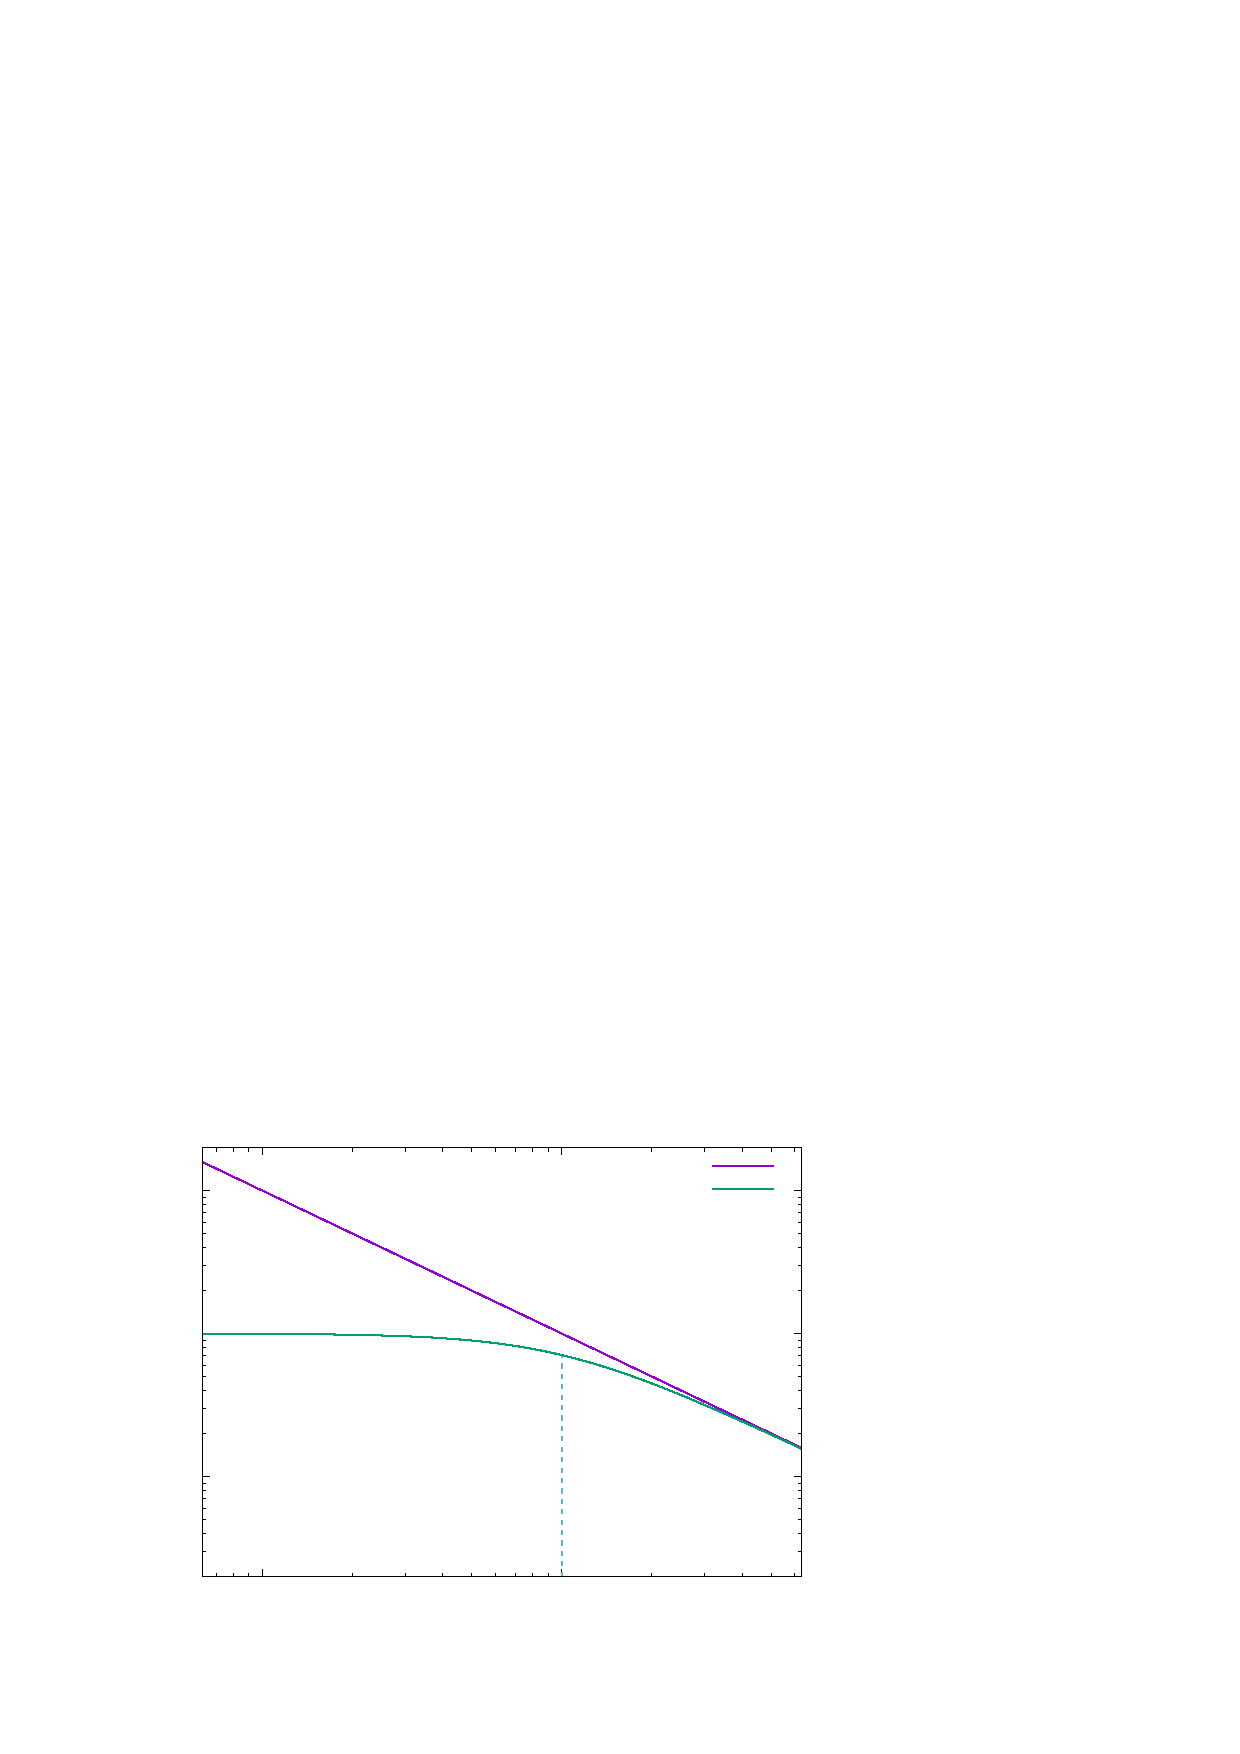
\includegraphics[width={360.00bp},height={252.00bp}]{integration2}}%
    \gplfronttext
  \end{picture}%
\endgroup
}
    \caption{Verlauf von $\hat{\nu}_1$ und $\hat{\nu}_2$ in Abhängigkeit von $\hat{\omega}$ mit der Grenzfrequenz $\omega_\text{int}$.}
\end{figure}
\newpage
\section{Differenzierschaltung}
\textbf{Durch die Differenzierschaltung in Abb. El2.4(b) werden nur Änderungen der Eingangsspannung verarbeitet.\\Zeigen Sie, dass gilt: 
\(U_a(t)=-R_2C_1\frac{dU_e}{dt}\) \\
Diskutieren Sie den Einfluss von $R_i$ und $C_i$ in Abb. El2.5(b) auf den Frequenzgang!}\\
Die Differenzierschaltung ist wie folgt aufgebaut:
\begin{figure}[h]
    \centering\begin{circuitikz}[european resistors]
        \draw(0,0) node[op amp, yscale=-1] (opamp){};
        \draw (opamp.+) to [C=$C_1$,-o,i_<=$I_1$] ++(-3,0) to [open,v>=$U_\text{e}$] ++(0,-3) to [short,o-] ++(2,0) to node[ground](gnd){} ++(0,0);
        \draw (opamp.-) to [short] ++(-1,0) to [short] ++(0,-1) to node[short](r2){} ++(0,0) to [short,-*] (gnd);
        \draw (gnd) to [short,-o]++(5.35,0) to node[short,-o](end){}++(0,0);
        \draw (opamp.out) to node[short,*-*](r1){} ++(1,0) to [short,-o] ++(1,0) to [open,v>=$U_\text{a}$] (end);
        %\draw (r1) to [short,*-,i>^=$I_2$]++(0,-1.5) to [R=$R_2$,v>=$U_2$] (r2);
        %\draw (r2)++(0,1) to [open] ++(-1,0) to node[short](o1){} ++(0,0)to[open,v>=$U_1$]++(0,-3);
        %\draw (o1) to [open,v^<=$U_3$]++(0,1);
        \draw (opamp.out) to [short,*-]++(0,2) to [R=$R_2$,i>=$I_2$]++(-2.35,0) to [short,-*] (opamp.+);
    \end{circuitikz}
    \caption{Schaltplan der Differenzierschaltung}
\end{figure}\\
Wie in der Aufgabe davor gilt:
\begin{align}
    I_1+I_2&=0\,\text{A}\\
    I_1&=C_1\cdot\dot{U}_\text{e}
\end{align}
Mit dem Ohm'schen Gesetz folgt für die Ausgangsspannung:
\begin{align}
    I_1&=-I_2\\
    C_1\cdot\dot{U}_\text{e}&=-\frac{U_\text{a}}{R_2}\\
    U_\text{a}&=-R_2C_1\cdot\dot{U}_\text{e}
\end{align}
Die Frequenzabhängigkeit ist gegeben durch:
\begin{align}
    U_\text{e}&=U_\text{e,0}\cdot e^{i\omega t}\\
    U_\text{a}&=-R_2C_1\cdot\dot{U}_\text{e}\\
    U_\text{a}&=-R_2C_1\cdot i\omega \cdot U_\text{e,0}\cdot e^{i\omega t}\\
    \nu_1&=\left|\frac{U_\text{a}}{U_\text{e}}\right|\\
    \nu_1&=\left|\frac{-R_2C_1\cdot i\omega \cdot U_\text{e,0}\cdot e^{i\omega t}}{U_\text{e,0}\cdot e^{i\omega t}}\right|\\
    \nu_1&=C_1R_2\omega
\end{align}\newpage
Nun wird auch die Differenzierschaltung nach folgenden Schaltplan erweitert:
\begin{figure}[h]
    \centering\begin{circuitikz}[european resistors]
        \draw(0,0) node[op amp, yscale=-1] (opamp){};
        \draw (opamp.+) to [C=$C_1$]++(-1.25,0)to [R=$R_1$] ++(-1.25,0) to [short,-o]+(-0.5,0)to[open,v>=$U_\text{e}$] ++(0,-3) to [short,o-] ++(2,0) to node[ground](gnd){} ++(0,0);
        \draw (opamp.-) to [short] ++(-1,0) to [short] ++(0,-1) to node[short](r2){} ++(0,0) to [short,-*] (gnd);
        \draw (gnd) to [short,-o]++(5.35,0) to node[short,-o](end){}++(0,0);
        \draw (opamp.out) to node[short,*-*](r1){} ++(1,0) to [short,-o] ++(1,0) to [open,v>=$U_\text{a}$] (end);
        %\draw (r1) to [short,*-,i>^=$I_2$]++(0,-1.5) to [R=$R_2$,v>=$U_2$] (r2);
        %\draw (r2)++(0,1) to [open] ++(-1,0) to node[short](o1){} ++(0,0)to[open,v>=$U_1$]++(0,-3);
        %\draw (o1) to [open,v^<=$U_3$]++(0,1);
        \draw (opamp.out) to [short,*-*]  ++(0,2) to node[short](R2){}++(0,0) to [R=$R_2$]++(-2.35,0) to [short,*-*] (opamp.+);
        \draw (R2) to [short,*-]++(0,1.5) to [C=$C_2$]++(-2.35,0) to [short,-*] ++(0,-1.5);
    \end{circuitikz}
    \caption{Schaltplan der erweiterten Differenzierschaltung}
\end{figure}\\
Zuerst wird betrachtet, wie sich der Widerstand $R_1$ auf die Verstärkung auswirkt.
Dazu wird das Verhältnis der ausgehenden und eingehenden Impedanz gebildet:
\begin{align}
    \nu_2&=\left|\frac{R_2}{R_1+\frac{1}{i\omega C_1}}\right|\\
    \nu_2&=\left|\frac{R_2}{R_1}\cdot\frac{1}{1+\frac{1}{i\omega C_1R_1}}\right|\\
    \nu_2&=\frac{R_2}{R_1}\cdot\left|\frac{i\omega C_1R_1}{i\omega C_1R_1+1}\right|\\
    \nu_2&=\frac{R_2}{R_1}\cdot\left|\frac{i\omega C_1R_1\cdot\left(1-i\omega C_1R_1\right)}{1+\omega C_1R_1}\right|\\
    \nu_2&=\frac{R_2}{R_1}\cdot\left|\frac{\omega C_1R_1\left(\omega C_1R_1+i\right)}{1+\omega C_1R_1}\right|\\
    \nu_2&=\frac{R_2}{R_1}\cdot\frac{\omega C_1R_1\cdot\sqrt{\omega C_1R_1+1}}{1+\omega C_1R_1}\\
    \nu_2&=\frac{R_2\omega C_1R_1}{R_1\cdot\sqrt{1+\omega C_1R_1}}
\end{align}
Nun werden wieder Überlegungen zur Grenzfrequenz getätigt und man kommt auf \citep[vgl.][S.448]{HBG}:
\begin{equation}
    \omega_\text{gr}=C_1R_1\omega=\omega_\text{diff}
\end{equation}
Es werden wieder, wie im Kapitel vorher, die dimensionslose Größen $\hat{\nu}$ und $\hat{\omega}$ gebildet:
\begin{align}
    \hat{\nu}_1(\hat{\omega})&=\hat{\omega}&\hat{\nu}_2(\hat{\omega})&=\frac{\hat{\omega}}{\sqrt{1+\left(\hat{\omega}\right)^2}}
\end{align}\newpage
Somit ergibt sich folgendes Diagramm:
\begin{figure}[h]
    \centering\scalebox{0.85}{% GNUPLOT: LaTeX picture with Postscript
\begingroup
  % Encoding inside the plot.  In the header of your document, this encoding
  % should to defined, e.g., by using
  % \usepackage[cp1252,<other encodings>]{inputenc}
  \inputencoding{cp1252}%
  \makeatletter
  \providecommand\color[2][]{%
    \GenericError{(gnuplot) \space\space\space\@spaces}{%
      Package color not loaded in conjunction with
      terminal option `colourtext'%
    }{See the gnuplot documentation for explanation.%
    }{Either use 'blacktext' in gnuplot or load the package
      color.sty in LaTeX.}%
    \renewcommand\color[2][]{}%
  }%
  \providecommand\includegraphics[2][]{%
    \GenericError{(gnuplot) \space\space\space\@spaces}{%
      Package graphicx or graphics not loaded%
    }{See the gnuplot documentation for explanation.%
    }{The gnuplot epslatex terminal needs graphicx.sty or graphics.sty.}%
    \renewcommand\includegraphics[2][]{}%
  }%
  \providecommand\rotatebox[2]{#2}%
  \@ifundefined{ifGPcolor}{%
    \newif\ifGPcolor
    \GPcolorfalse
  }{}%
  \@ifundefined{ifGPblacktext}{%
    \newif\ifGPblacktext
    \GPblacktexttrue
  }{}%
  % define a \g@addto@macro without @ in the name:
  \let\gplgaddtomacro\g@addto@macro
  % define empty templates for all commands taking text:
  \gdef\gplbacktext{}%
  \gdef\gplfronttext{}%
  \makeatother
  \ifGPblacktext
    % no textcolor at all
    \def\colorrgb#1{}%
    \def\colorgray#1{}%
  \else
    % gray or color?
    \ifGPcolor
      \def\colorrgb#1{\color[rgb]{#1}}%
      \def\colorgray#1{\color[gray]{#1}}%
      \expandafter\def\csname LTw\endcsname{\color{white}}%
      \expandafter\def\csname LTb\endcsname{\color{black}}%
      \expandafter\def\csname LTa\endcsname{\color{black}}%
      \expandafter\def\csname LT0\endcsname{\color[rgb]{1,0,0}}%
      \expandafter\def\csname LT1\endcsname{\color[rgb]{0,1,0}}%
      \expandafter\def\csname LT2\endcsname{\color[rgb]{0,0,1}}%
      \expandafter\def\csname LT3\endcsname{\color[rgb]{1,0,1}}%
      \expandafter\def\csname LT4\endcsname{\color[rgb]{0,1,1}}%
      \expandafter\def\csname LT5\endcsname{\color[rgb]{1,1,0}}%
      \expandafter\def\csname LT6\endcsname{\color[rgb]{0,0,0}}%
      \expandafter\def\csname LT7\endcsname{\color[rgb]{1,0.3,0}}%
      \expandafter\def\csname LT8\endcsname{\color[rgb]{0.5,0.5,0.5}}%
    \else
      % gray
      \def\colorrgb#1{\color{black}}%
      \def\colorgray#1{\color[gray]{#1}}%
      \expandafter\def\csname LTw\endcsname{\color{white}}%
      \expandafter\def\csname LTb\endcsname{\color{black}}%
      \expandafter\def\csname LTa\endcsname{\color{black}}%
      \expandafter\def\csname LT0\endcsname{\color{black}}%
      \expandafter\def\csname LT1\endcsname{\color{black}}%
      \expandafter\def\csname LT2\endcsname{\color{black}}%
      \expandafter\def\csname LT3\endcsname{\color{black}}%
      \expandafter\def\csname LT4\endcsname{\color{black}}%
      \expandafter\def\csname LT5\endcsname{\color{black}}%
      \expandafter\def\csname LT6\endcsname{\color{black}}%
      \expandafter\def\csname LT7\endcsname{\color{black}}%
      \expandafter\def\csname LT8\endcsname{\color{black}}%
    \fi
  \fi
    \setlength{\unitlength}{0.0500bp}%
    \ifx\gptboxheight\undefined%
      \newlength{\gptboxheight}%
      \newlength{\gptboxwidth}%
      \newsavebox{\gptboxtext}%
    \fi%
    \setlength{\fboxrule}{0.5pt}%
    \setlength{\fboxsep}{1pt}%
\begin{picture}(7200.00,5040.00)%
    \gplgaddtomacro\gplbacktext{%
      \csname LTb\endcsname%%
      \put(814,1610){\makebox(0,0)[r]{\strut{}$0.1$}}%
      \put(814,2905){\makebox(0,0)[r]{\strut{}$1$}}%
      \put(814,4201){\makebox(0,0)[r]{\strut{}$10$}}%
      \put(1563,484){\makebox(0,0){\strut{}$0.1$}}%
      \put(4343,484){\makebox(0,0){\strut{}$1$}}%
    }%
    \gplgaddtomacro\gplfronttext{%
      \csname LTb\endcsname%%
      \put(209,2761){\rotatebox{-270}{\makebox(0,0){\strut{}$\hat{\nu}\left(\hat{\omega}\right)$}}}%
      \csname LTb\endcsname%%
      \put(6748,2761){\rotatebox{-270}{\makebox(0,0){\strut{}}}}%
      \csname LTb\endcsname%%
      \put(3819,154){\makebox(0,0){\strut{}$\hat{\omega}$}}%
      \csname LTb\endcsname%%
      \put(3819,4819){\makebox(0,0){\strut{}}}%
      \csname LTb\endcsname%%
      \put(132,-110){\makebox(0,0)[l]{\strut{}}}%
      \csname LTb\endcsname%%
      \put(5706,4646){\makebox(0,0)[r]{\strut{}$\hat{\nu}_1(\hat{\omega})$}}%
      \csname LTb\endcsname%%
      \put(5706,4426){\makebox(0,0)[r]{\strut{}$\hat{\nu}_2(\hat{\omega})$}}%
      \csname LTb\endcsname%%
      \put(3819,54658){\makebox(0,0){\strut{}}}%
    }%
    \gplbacktext
    \put(0,0){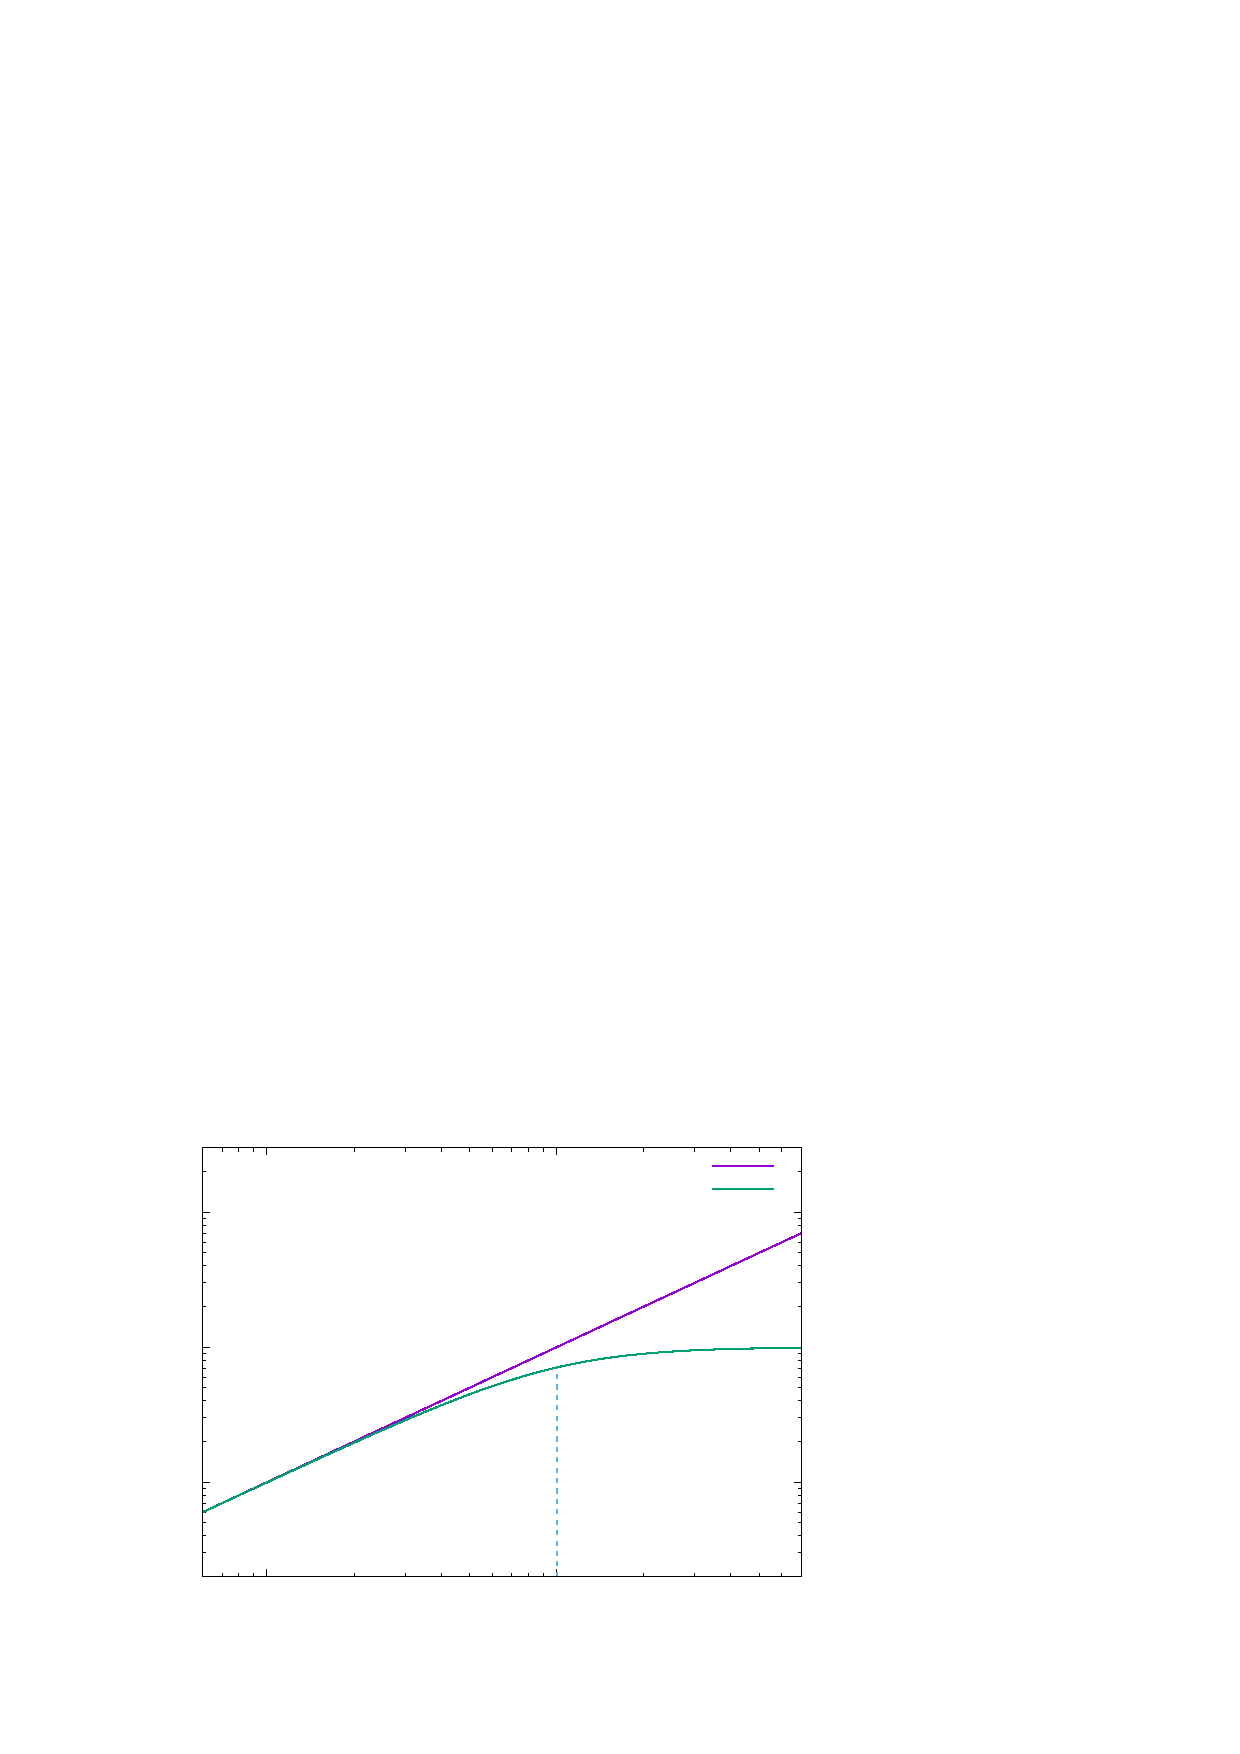
\includegraphics[width={360.00bp},height={252.00bp}]{differentiation2}}%
    \gplfronttext
  \end{picture}%
\endgroup
}
    \caption{Verlauf von $\hat{\nu}_1$ und $\hat{\nu}_2$ in Abhängigkeit von $\hat{\omega}$ mit der Grenzfrequenz $\omega_\text{diff}$.}
\end{figure}\\
Es fällt auf, dass dieses dem Diagramm der Integrationsschaltung ziemlich ähnlich sieht. Beide sind zueinander achsensymmetrisch.\\\\
Nun wird auch noch der Kondensator $C_2$ mitbetrachtet.
Die erhaltene Schaltung wird auch Bandpass genannt.
Diese ist eine Reihenschaltung eines Hochpass- (Integrationsschaltung) und Tiefpassfilters (Differenzierschaltung).\\
Um die Verstärkung zu bekommen, wird wieder das Verhältnis der Impedanzen berechnet:
\begin{align}
    \nu&=\left|\frac{\frac{1}{\frac{1}{R_2}+i\omega C_2}}{R_1+\frac{1}{i\omega C_1}}\right|\\
    \nu&=\left|\frac{R_2}{1+R_2i\omega C_2}\cdot\frac{i\omega C_1}{R_1i\omega C_1+1}\right|\\
    \nu&=\left|\frac{R_2}{R_1}\cdot\frac{1}{1+R_2i\omega C_2}\cdot\frac{R_1i\omega C_1}{R_1i\omega C_1+1}\right|\\
    \nu&=\frac{R_2}{R_1}\cdot\left|\frac{\left(1-R_2i\omega C_2\right)}{1+\left(R_2\omega C_2\right)^2}\cdot\frac{R_1i\omega C_1\cdot\left(1-iR_1C_1\omega\right)}{\left(R_1\omega C_1\right)^2+1}\right|\\
    \nu&=\frac{R_2}{R_1}\cdot\frac{\sqrt{1+\left(R_2\omega C_2\right)^2}}{1+\left(R_2\omega C_2\right)^2}\cdot\frac{\left(R_1\omega C_1\right)\sqrt{1+\left(R_1C_1\omega\right)^2}}{\left(R_1\omega C_1\right)^2+1}\\
    \nu&=\frac{R_2}{R_1}\cdot\frac{1}{\sqrt{1+\left(R_2\omega C_2\right)^2}}\cdot\frac{\left(R_1\omega C_1\right)}{\sqrt{1+\left(R_1C_1\omega\right)^2}}\\
    \nu&=\frac{R_2}{R_1}\cdot\frac{\left(R_1\omega C_1\right)}{\sqrt{1+\left(R_1\omega C_1\right)^2+\left(R_2\omega C_2\right)^2+\left(R_1\omega C_1\right)^2\left(R_2\omega C_2\right)^2}}\\
    \nu&=\frac{R_2}{R_1}\cdot\frac{1}{\sqrt{\frac{1}{\left(R_1\omega C_1\right)^2}+1+\frac{\left(R_2C_2\right)^2}{\left(R_1C_1\right)^2}+\left(R_2\omega C_2\right)^2}}
\end{align}
\begin{align}
    \nu&=\frac{1}{\sqrt{\frac{1}{\left(R_2\omega C_1\right)^2}+\left(\frac{R_1}{R_2}\right)^2+\left(\frac{C_2}{C_1}\right)^2+\left(R_1\omega C_2\right)^2}}\\
    \nu&=\frac{1}{\sqrt{\frac{1}{\left(R_2\omega C_1\right)^2}+\left(\frac{R_1}{R_2}\right)^2+\left(\frac{C_2}{C_1}\right)^2+\left(R_1\omega C_2\right)^2+2\frac{R_1C_2}{R_2C_1}-2\frac{R_1C_2}{R_2C_1}}}\\
    \nu&=\frac{1}{\sqrt{\left(R_1\omega C_2-\frac{1}{R_2\omega C_1}\right)^2+\left(\frac{R_1}{R_2}+\frac{C_2}{C_1}\right)^2}}\\
\end{align}
Man definiet sich eine Mittelfrequenz $\omega_\text{m}$, welche der geometrische Mittelwert der beiden Grenzfrequenzen ist:
\begin{equation}
    \omega_\text{m}=\sqrt{\omega_\text{int}\cdot\omega_\text{diff}}
\end{equation}
Die Differenz der beiden Grenzfrequenzen wird Bandbreite genannt.
Der Bandpass hat eine (nahezu) konstante Verstärkung für Frequenzen, welche in der Bandbreite liegen \citep[vgl.][S.454]{HBG}.
Skizziert man nun die Verstärkung des Bandpasses, so erhält man:
\begin{figure}[h]
    \center\scalebox{0.85}{% GNUPLOT: LaTeX picture with Postscript
\begingroup
  % Encoding inside the plot.  In the header of your document, this encoding
  % should to defined, e.g., by using
  % \usepackage[cp1252,<other encodings>]{inputenc}
  \inputencoding{cp1252}%
  \makeatletter
  \providecommand\color[2][]{%
    \GenericError{(gnuplot) \space\space\space\@spaces}{%
      Package color not loaded in conjunction with
      terminal option `colourtext'%
    }{See the gnuplot documentation for explanation.%
    }{Either use 'blacktext' in gnuplot or load the package
      color.sty in LaTeX.}%
    \renewcommand\color[2][]{}%
  }%
  \providecommand\includegraphics[2][]{%
    \GenericError{(gnuplot) \space\space\space\@spaces}{%
      Package graphicx or graphics not loaded%
    }{See the gnuplot documentation for explanation.%
    }{The gnuplot epslatex terminal needs graphicx.sty or graphics.sty.}%
    \renewcommand\includegraphics[2][]{}%
  }%
  \providecommand\rotatebox[2]{#2}%
  \@ifundefined{ifGPcolor}{%
    \newif\ifGPcolor
    \GPcolorfalse
  }{}%
  \@ifundefined{ifGPblacktext}{%
    \newif\ifGPblacktext
    \GPblacktexttrue
  }{}%
  % define a \g@addto@macro without @ in the name:
  \let\gplgaddtomacro\g@addto@macro
  % define empty templates for all commands taking text:
  \gdef\gplbacktext{}%
  \gdef\gplfronttext{}%
  \makeatother
  \ifGPblacktext
    % no textcolor at all
    \def\colorrgb#1{}%
    \def\colorgray#1{}%
  \else
    % gray or color?
    \ifGPcolor
      \def\colorrgb#1{\color[rgb]{#1}}%
      \def\colorgray#1{\color[gray]{#1}}%
      \expandafter\def\csname LTw\endcsname{\color{white}}%
      \expandafter\def\csname LTb\endcsname{\color{black}}%
      \expandafter\def\csname LTa\endcsname{\color{black}}%
      \expandafter\def\csname LT0\endcsname{\color[rgb]{1,0,0}}%
      \expandafter\def\csname LT1\endcsname{\color[rgb]{0,1,0}}%
      \expandafter\def\csname LT2\endcsname{\color[rgb]{0,0,1}}%
      \expandafter\def\csname LT3\endcsname{\color[rgb]{1,0,1}}%
      \expandafter\def\csname LT4\endcsname{\color[rgb]{0,1,1}}%
      \expandafter\def\csname LT5\endcsname{\color[rgb]{1,1,0}}%
      \expandafter\def\csname LT6\endcsname{\color[rgb]{0,0,0}}%
      \expandafter\def\csname LT7\endcsname{\color[rgb]{1,0.3,0}}%
      \expandafter\def\csname LT8\endcsname{\color[rgb]{0.5,0.5,0.5}}%
    \else
      % gray
      \def\colorrgb#1{\color{black}}%
      \def\colorgray#1{\color[gray]{#1}}%
      \expandafter\def\csname LTw\endcsname{\color{white}}%
      \expandafter\def\csname LTb\endcsname{\color{black}}%
      \expandafter\def\csname LTa\endcsname{\color{black}}%
      \expandafter\def\csname LT0\endcsname{\color{black}}%
      \expandafter\def\csname LT1\endcsname{\color{black}}%
      \expandafter\def\csname LT2\endcsname{\color{black}}%
      \expandafter\def\csname LT3\endcsname{\color{black}}%
      \expandafter\def\csname LT4\endcsname{\color{black}}%
      \expandafter\def\csname LT5\endcsname{\color{black}}%
      \expandafter\def\csname LT6\endcsname{\color{black}}%
      \expandafter\def\csname LT7\endcsname{\color{black}}%
      \expandafter\def\csname LT8\endcsname{\color{black}}%
    \fi
  \fi
    \setlength{\unitlength}{0.0500bp}%
    \ifx\gptboxheight\undefined%
      \newlength{\gptboxheight}%
      \newlength{\gptboxwidth}%
      \newsavebox{\gptboxtext}%
    \fi%
    \setlength{\fboxrule}{0.5pt}%
    \setlength{\fboxsep}{1pt}%
\begin{picture}(7200.00,5040.00)%
    \gplgaddtomacro\gplbacktext{%
      \csname LTb\endcsname%%
      \put(682,704){\makebox(0,0)[r]{\strut{}$0$}}%
      \put(682,1527){\makebox(0,0)[r]{\strut{}$2$}}%
      \put(682,2350){\makebox(0,0)[r]{\strut{}$4$}}%
      \put(682,3173){\makebox(0,0)[r]{\strut{}$6$}}%
      \put(682,3996){\makebox(0,0)[r]{\strut{}$8$}}%
      \put(682,4819){\makebox(0,0)[r]{\strut{}$10$}}%
      \put(814,484){\makebox(0,0){\strut{}$0.0001$}}%
      \put(1549,484){\makebox(0,0){\strut{}$0.001$}}%
      \put(2284,484){\makebox(0,0){\strut{}$0.01$}}%
      \put(3019,484){\makebox(0,0){\strut{}$0.1$}}%
      \put(3754,484){\makebox(0,0){\strut{}$1$}}%
      \put(4488,484){\makebox(0,0){\strut{}$10$}}%
      \put(5223,484){\makebox(0,0){\strut{}$100$}}%
      \put(5958,484){\makebox(0,0){\strut{}$1000$}}%
      \put(6693,484){\makebox(0,0){\strut{}$10000$}}%
    }%
    \gplgaddtomacro\gplfronttext{%
      \csname LTb\endcsname%%
      \put(209,2761){\rotatebox{-270}{\makebox(0,0){\strut{}$\hat{\nu}$}}}%
      \csname LTb\endcsname%%
      \put(6748,2761){\rotatebox{-270}{\makebox(0,0){\strut{}}}}%
      \csname LTb\endcsname%%
      \put(3753,154){\makebox(0,0){\strut{}$\hat{\omega}$}}%
      \csname LTb\endcsname%%
      \put(3753,4819){\makebox(0,0){\strut{}}}%
      \csname LTb\endcsname%%
      \put(132,-110){\makebox(0,0)[l]{\strut{}}}%
      \csname LTb\endcsname%%
      \put(3753,13807){\makebox(0,0){\strut{}}}%
    }%
    \gplbacktext
    \put(0,0){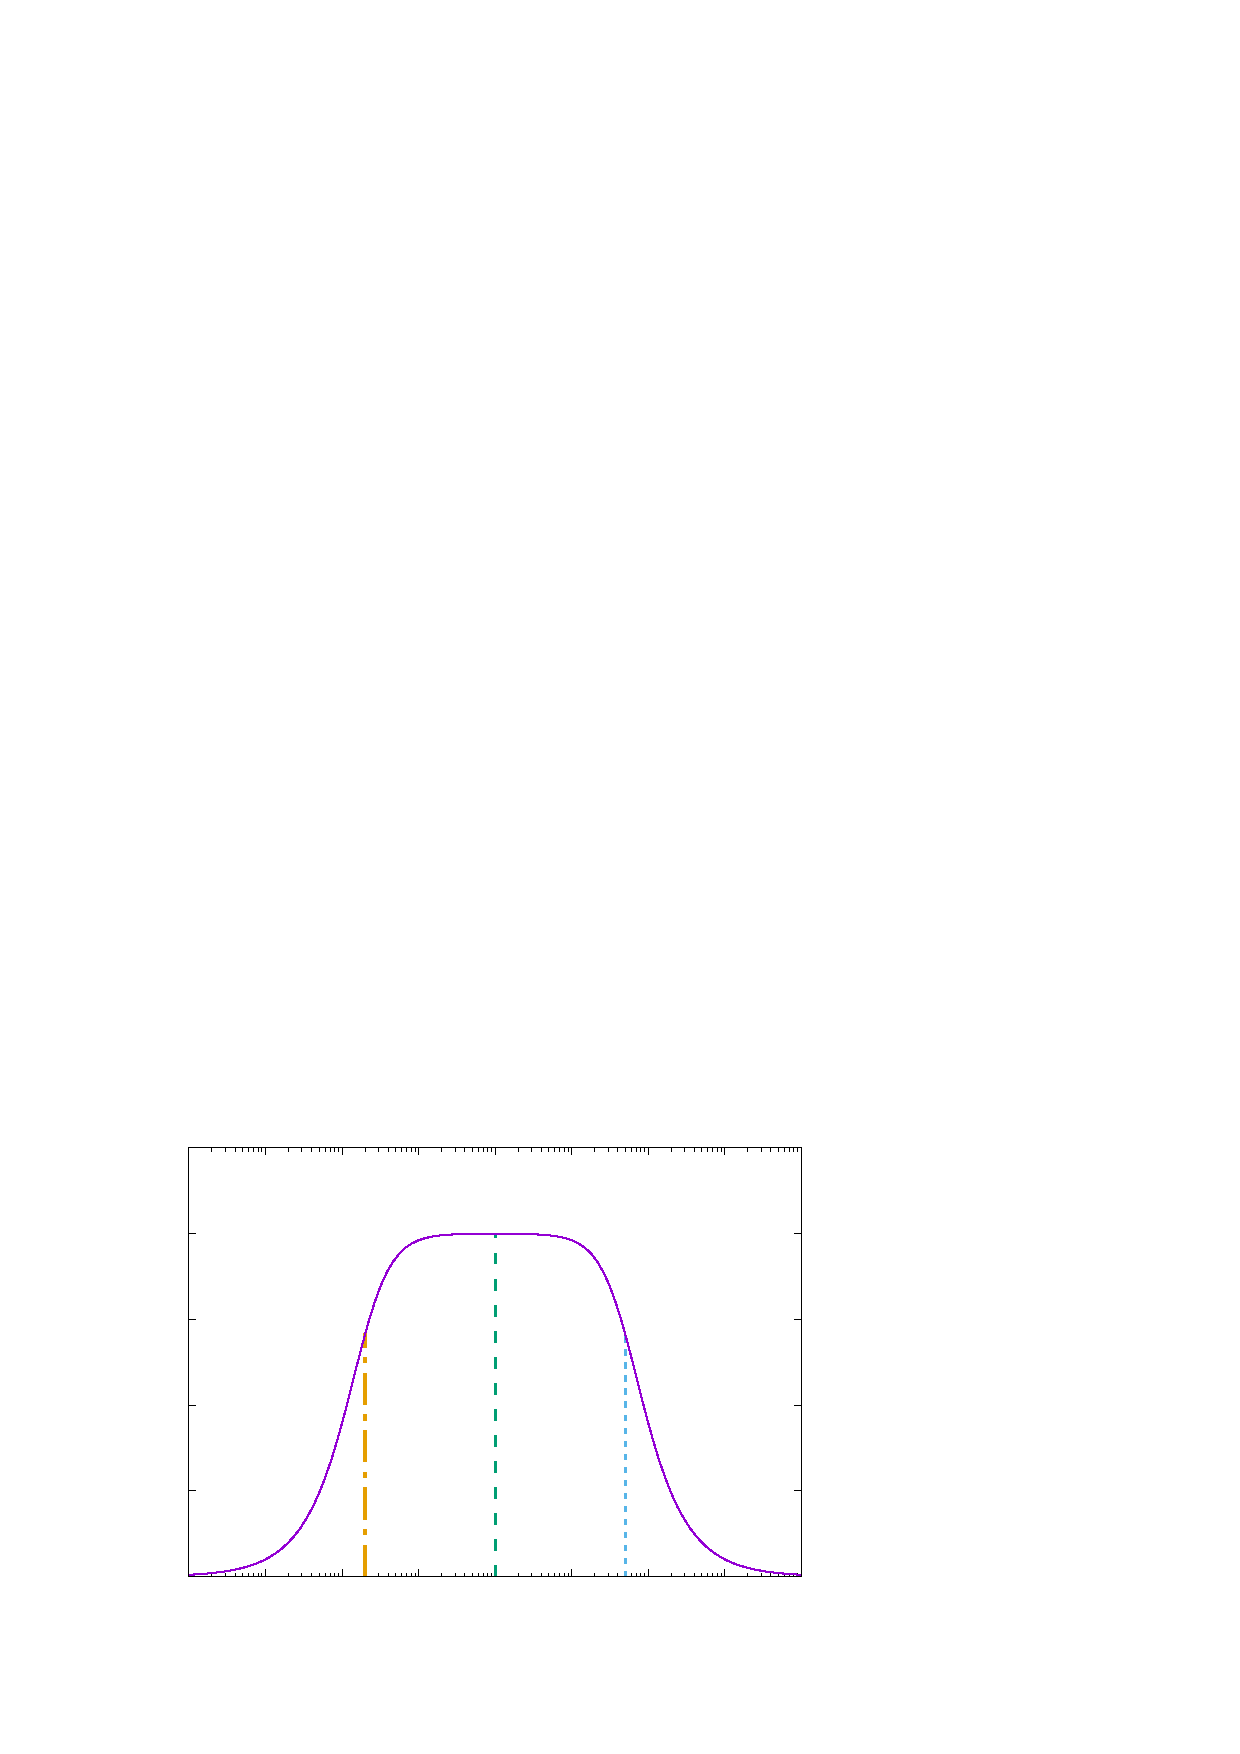
\includegraphics[width={360.00bp},height={252.00bp}]{bandpass3}}%
    \gplfronttext
  \end{picture}%
\endgroup
}
    \caption{Verlauf des Bandpasses mit $R_1=0,05\,\Omega$, $R_2=100\,\Omega$,$C_1=4\,\text{F}$ und $C_2=0,5\,\text{F}$}
\end{figure}\\
Man erkennt, dass unterhalb der Grenzfrequenz $\omega_\text{diff}$ (gelb) der Bandpass wie eine Differenzierschaltung fungiert und über der Grenzfrequenz $\omega_\text{int}$ (blau) wie ein Integrationsschaltung.
Die Mittelfrequenz $\omega_\text{m}$ (grün) liegt zwischen $\omega_\text{diff}$ und $\omega_\text{int}$.
Um diese herum, fungiert der Bandpass als normaler Verstärker.